\documentclass{article}
\usepackage[utf8]{inputenc}
\usepackage{tikz}
\usepackage{graphicx}
\usetikzlibrary{calc}
\title{Harnessing the Master Algorithm: Strategies for AI Large Language Models to Mitigate Hallucinations}
\author{
  Hallucinated Pedro Domingos\\
  \texttt{first1.last1@xxxxx.com}
  \and
  Howard, Bion\\
  \texttt{first2.last2@xxxxx.com}
}
\date{Christmas Eve 2023}

\begin{document}

\maketitle

\begin{figure}[h]
\centering
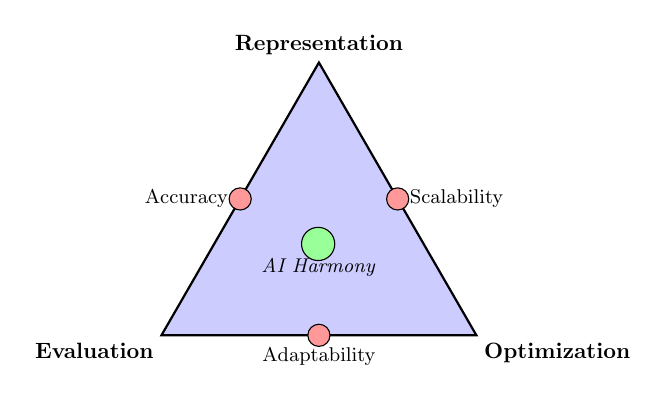
\begin{tikzpicture}[scale=2, every node/.style={scale=0.8}]
  \path 
    (0,0) coordinate (A)
    -- (60:2cm) coordinate (B)
    -- (2cm,0) coordinate (C)
    -- cycle;
  \draw[thick, fill=blue!20] (A) -- (B) -- (C) -- cycle;
  
  % Label corners
  \node at (B) [above, font=\bfseries] {Representation};
  \node at (A) [below left, font=\bfseries] {Evaluation};
  \node at (C) [below right, font=\bfseries] {Optimization};
  
  % Label midpoints
  \draw[fill=red!40] 
    ($(A)!0.5!(B)$) circle (2pt) node[left=2pt, font=\small] {Accuracy}
    ($(B)!0.5!(C)$) circle (2pt) node[right=2pt, font=\small] {Scalability}
    ($(C)!0.5!(A)$) circle (2pt) node[below=2pt, font=\small] {Adaptability};

  % Add center point
  \draw[fill=green!40] 
    ($(A)!0.5!(B)!0.33!(C)$) circle (3pt) node[below=3pt, font=\small\itshape] {AI Harmony};
\end{tikzpicture}
\caption{Intersection of Representation, Evaluation, and Optimization in AI.}
\label{fig:master-algorithm-triangle}
\end{figure}

\begin{abstract}
In this review, we explore innovative approaches for Large Language Models (LLMs) in mitigating the phenomenon of 'hallucinations', leveraging the principles of the Master Algorithm: Representation, Evaluation, and Optimization. By examining the intersection of cognitive science and machine learning, we propose a multifaceted framework aimed at enhancing the accuracy, reliability, and contextual awareness of LLMs. Our analysis synthesizes recent advancements in AI research, emphasizing the need for dynamic representational models, robust evaluation metrics, and continuous optimization processes.
\end{abstract}

\newpage

\tableofcontents

\newpage

\section{Introduction}
The advent of Large Language Models (LLMs) in the realm of artificial intelligence has brought significant advancements but also challenges, notably the phenomenon of 'hallucinations' or generating misleading or false information. Understanding and mitigating these hallucinations is critical for the continued growth and reliability of LLMs. This paper reviews strategies rooted in the Master Algorithm's principles: Representation, Evaluation, and Optimization, to address this challenge.

\section{Representation in LLMs}
\subsection{Current Representational Models}
Current representational models in Large Language Models (LLMs) have predominantly focused on neural network architectures, especially transformers, to interpret and generate human language. However, these models often lack the ability to fully capture the nuances and context of human communication.

\subsection{Incorporating Cognitive Structures}
Incorporating cognitive structures into LLMs involves integrating concepts from cognitive science, such as memory systems and learning processes, into AI models. This approach aims to improve the contextual awareness and adaptability of LLMs.

\subsection{Conceptual Diagrams of Advanced Representational Models}
% Assuming you have DALL-E generated diagrams as images
\begin{figure}[h]
\centering
\includegraphics[width=0.8\textwidth]{advanced_rep_models.png}
\caption{DALL-E generated conceptual diagrams of advanced representational models in LLMs.}
\label{fig:advanced-rep-models}
\end{figure}

\section{Evaluation Strategies}
\subsection{Existing Evaluation Metrics for LLMs}
Traditional metrics for evaluating LLMs, such as perplexity and BLEU score, primarily focus on linguistic accuracy. Recent developments suggest the need for more holistic evaluation metrics that encompass contextual understanding and ethical considerations.

\subsection{Integrating Contextual and Ethical Considerations}
This subsection explores how integrating contextual and ethical considerations into evaluation metrics can enhance the overall effectiveness and societal impact of LLMs.

\subsection{Case Studies: Evaluation in Practice}
Case studies highlighting the implementation of these novel evaluation strategies in real-world scenarios.

\section{Optimization Techniques}
\subsection{Continuous Learning Models}
Continuous learning models enable LLMs to adapt and evolve over time, learning from new data and interactions to improve their performance and reduce hallucinations.

\subsection{Adaptive Algorithms for Real-time Adjustments}
Discussion on the development and application of adaptive algorithms that allow LLMs to make real-time adjustments for better accuracy and contextuality.

\subsection{Performance Metrics Pre- and Post-Optimization}
% Assuming you have data analysis figures
\begin{figure}[h]
\centering

\caption{Python-driven analysis of LLM performance metrics before and after optimization.}
\label{fig:performance-metrics}
\end{figure}

\section{Interdisciplinary Insights}
\subsection{Cognitive Science and AI: A Symbiotic Relationship}
Exploring the symbiotic relationship between cognitive science and AI, and how this interplay can lead to more advanced and human-like AI systems.

\subsection{Learning from Human Cognitive Processes}
Delving into how AI can benefit from understanding and mimicking human cognitive processes, particularly in the context of language understanding and generation.

\section{Challenges and Future Directions}
\subsection{Addressing Current Limitations}
A critical analysis of the current limitations in LLM technology, particularly focusing on the challenges of scalability, ethical use, and the mitigation of biases.

\subsection{The Road Ahead: Ethical and Practical Considerations}
This subsection discusses the ethical and practical considerations that must guide future developments in LLM technology, emphasizing responsible AI development.

\section{Conclusion}
\subsection{Summarizing Key Findings}
A summary of the key findings from the article, highlighting the advances in LLMs through the integration of Representation, Evaluation, and Optimization.

\subsection{The Next Steps in AI Development}
Outlining the next steps in AI development, focusing on continued interdisciplinary collaboration and the pursuit of ethically aligned, context-aware AI systems.

% Add any additional acknowledgments, references, or appendices here

\end{document}